%%%%%%%%%%%%%%%%%%%%%%%%%%%%%%%%%%%%%%%%%%%%%%%%%%%%%%%%%%%%%%%%%%%%%%%%%%%%%%%%
%2345678901234567890123456789012345678901234567890123456789012345678901234567890
%        1         2         3         4         5         6         7         8

% \documentclass[letterpaper, 10 pt, conference]{ieeeconf}  % Comment this line out if you need a4paper

\documentclass[a4paper, 10pt, conference]{ieeeconf}      % Use this line for a4 paper

\IEEEoverridecommandlockouts                              % This command is only needed if
                                                          % you want to use the \thanks command

\overrideIEEEmargins                                      % Needed to meet printer requirements.

%In case you encounter the following error:
%Error 1010 The PDF file may be corrupt (unable to open PDF file) OR
%Error 1000 An error occurred while parsing a contents stream. Unable to analyze the PDF file.
%This is a known problem with pdfLaTeX conversion filter. The file cannot be opened with acrobat reader
%Please use one of the alternatives below to circumvent this error by uncommenting one or the other
%\pdfobjcompresslevel=0
%\pdfminorversion=4

% See the \addtolength command later in the file to balance the column lengths
% on the last page of the document

% The following packages can be found on http:\\www.ctan.org
\usepackage{graphics} % for pdf, bitmapped graphics files
\usepackage{epsfig} % for postscript graphics files
\usepackage{mathptmx} % assumes new font selection scheme installed
\usepackage{times} % assumes new font selection scheme installed
\usepackage{amsmath} % assumes amsmath package installed
\usepackage{amssymb}  % assumes amsmath package installed

\title{\LARGE \bf
A comparative analysis of the main robotic open-source simulation tools*
}


% \author{Albert Author$^{1}$ and Bernard D. Researcher$^{2}$% <-this % stops a space
\author{Jose Luis Blanco-Claraco$^{1}$ and Francisco J. Mañas-Alvarez$^{2}$% <-this % stops a space
\thanks{*This work was not supported by any organization}% <-this % stops a space
\thanks{$^{1}$Jose Luis Blanco-Claraco is with Engineering Department, University of Almería, Agrifood Campus of International Excellence (ceiA3), and CIESOL, 04120 Almería, Spain
        {\tt\small jlblanco@ual.es}}%
\thanks{$^{2}$Francisco J. Mañas-Alvarez with the Department of Computer Sciences and Automatic Control, Universidad Nacional de Educación a Distancia (UNED), Madrid, Spain
        {\tt\small fjmanas@dia.uned.es}}%
}


\begin{document}



\maketitle
\thispagestyle{empty}
\pagestyle{empty}


%%%%%%%%%%%%%%%%%%%%%%%%%%%%%%%%%%%%%%%%%%%%%%%%%%%%%%%%%%%%%%%%%%%%%%%%%%%%%%%%
\begin{abstract}

This electronic document is a live template. The various components of your paper [title, text, heads, etc.] are already defined on the style sheet, as illustrated by the portions given in this document.

\end{abstract}


%%%%%%%%%%%%%%%%%%%%%%%%%%%%%%%%%%%%%%%%%%%%%%%%%%%%%%%%%%%%%%%%%%%%%%%%%%%%%%%%
\section{INTRODUCTION}

Review: \cite{collins2021review}

MVSIM: \cite{blanco2023multivehicle}\\
Gazebo: \cite{koenig2004design}\\
Webots: \cite{michel2004cyberbotics}\\

Introducción\\
Contribuciones\\
Estructura\\
Límite de 6 páginas

\section{The simulators}
\subsection{Gazebo}
TO-DO. Fig. \ref{fig:Gazebo}.
\begin{figure}[thpb]
	\centering
    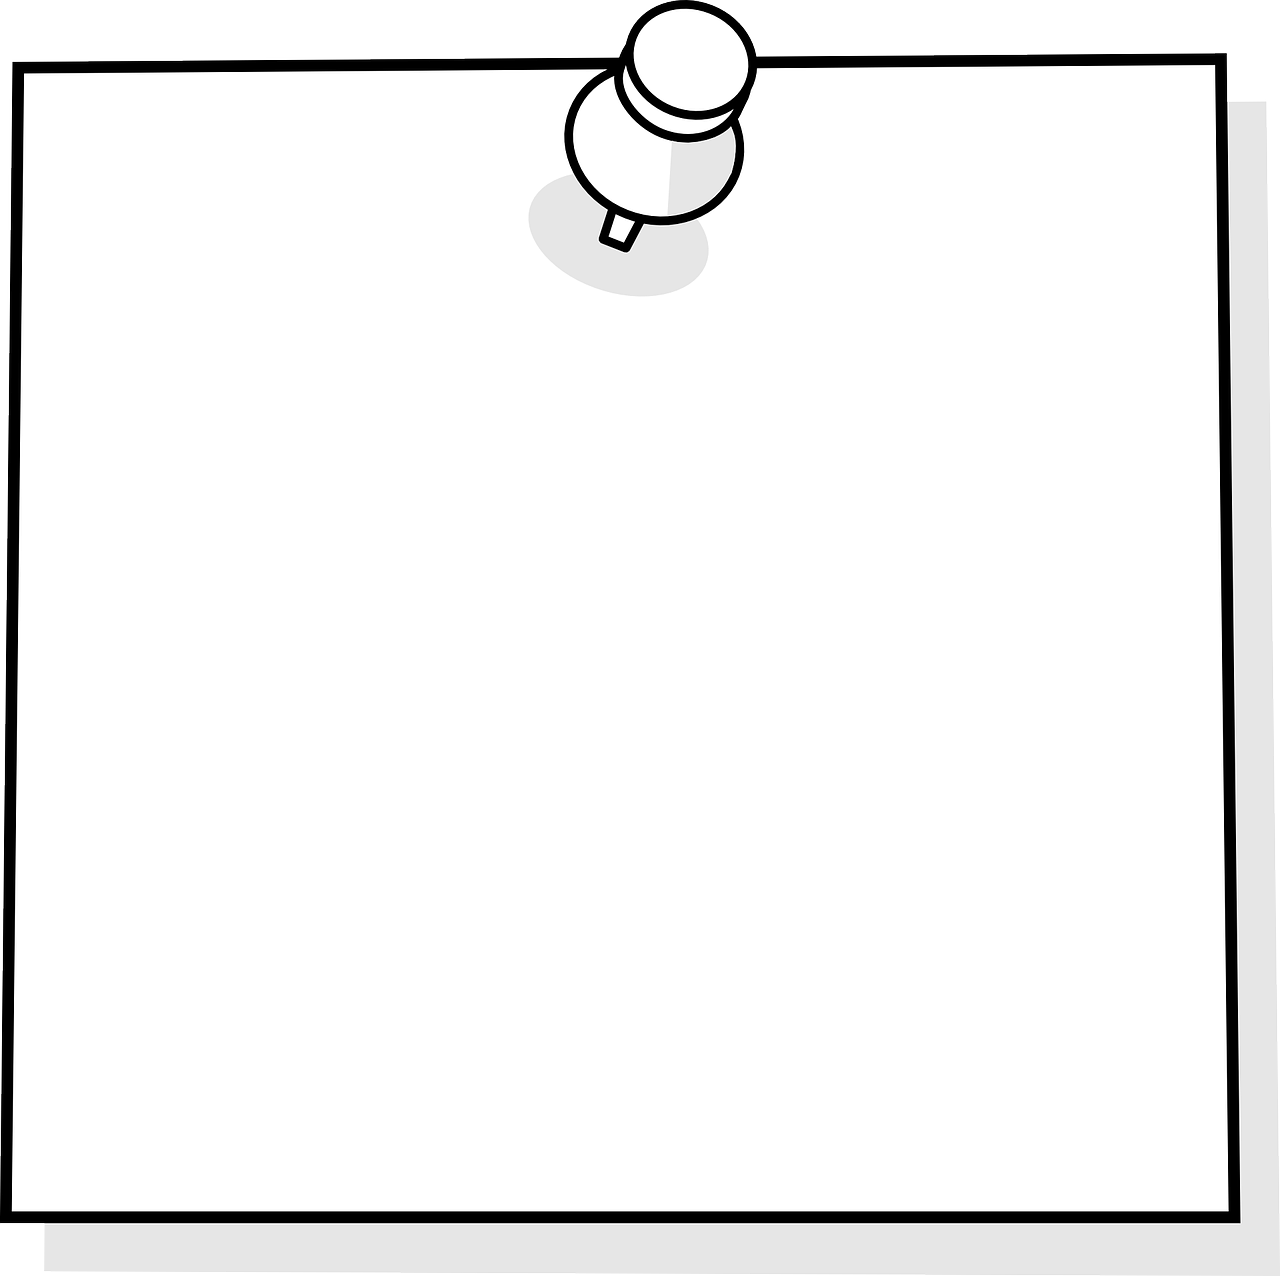
\includegraphics[width=0.7\columnwidth]{figs/example.png}
    \caption{Gazebo Simulation Interface}
    \label{fig:Gazebo}
\end{figure}
\subsection{Webots}
TO-DO. Fig. \ref{fig:Webots}.
\begin{figure}[thpb]
	\centering
    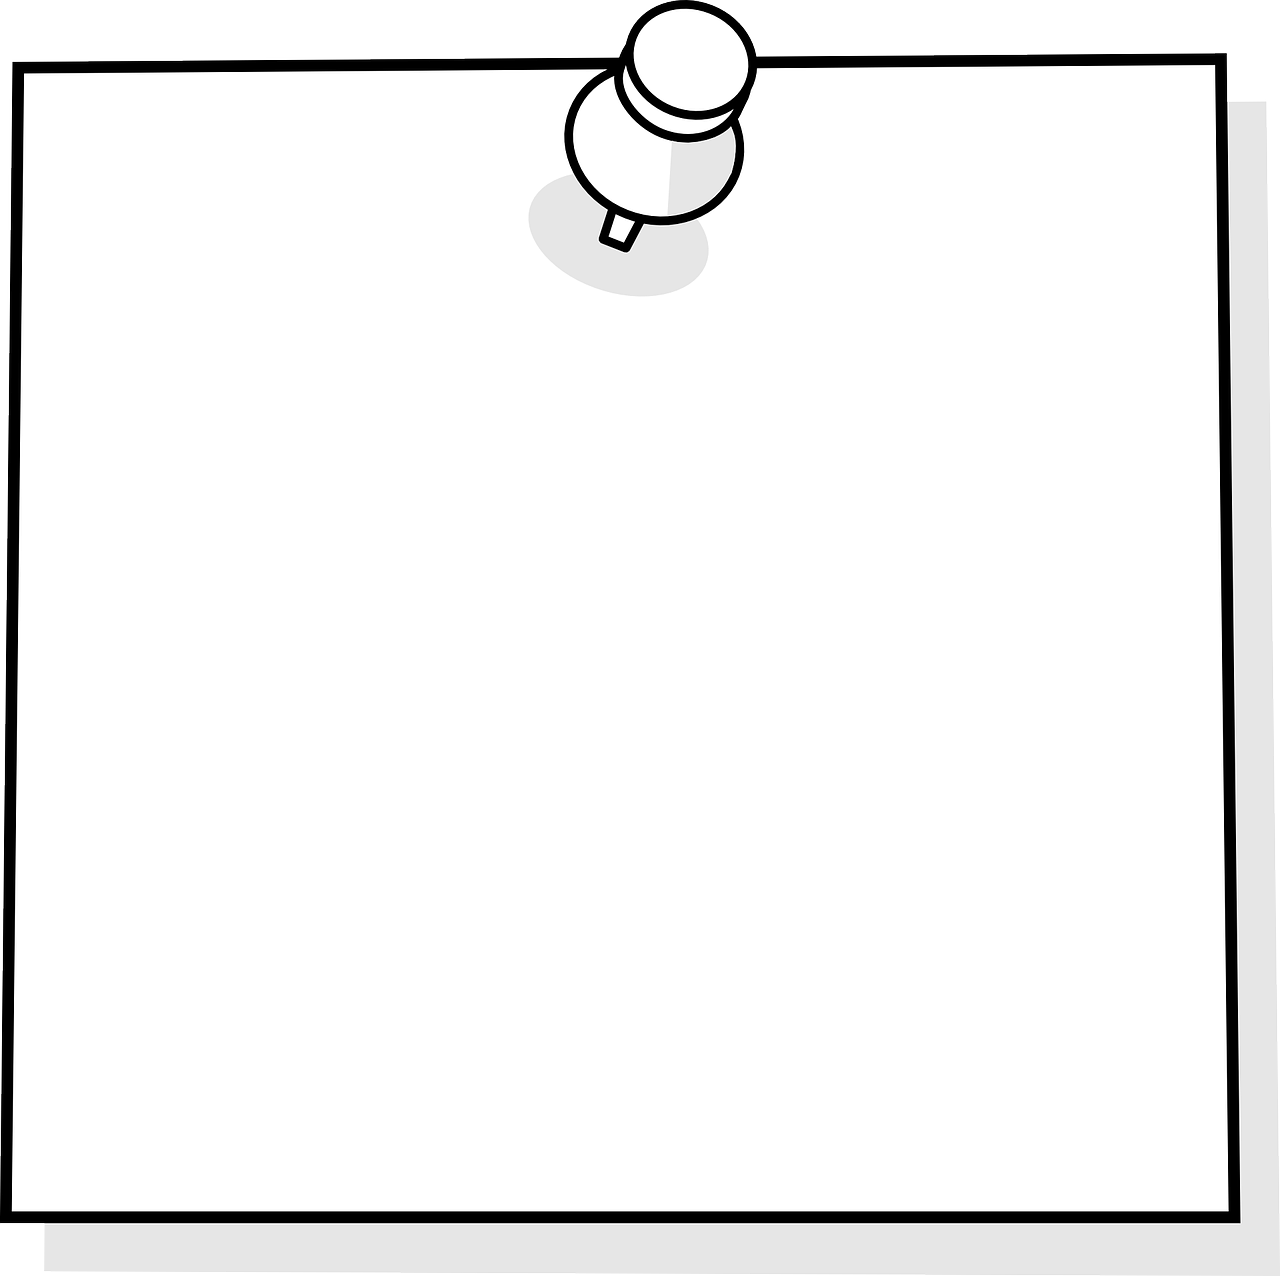
\includegraphics[width=0.7\columnwidth]{figs/example.png}
    \caption{Webots Simulation Interface}
    \label{fig:Webots}
\end{figure}
\subsection{MVSIM}
TO-DO. Fig. \ref{fig:MVSIM}.
\begin{figure}[thpb]
	\centering
    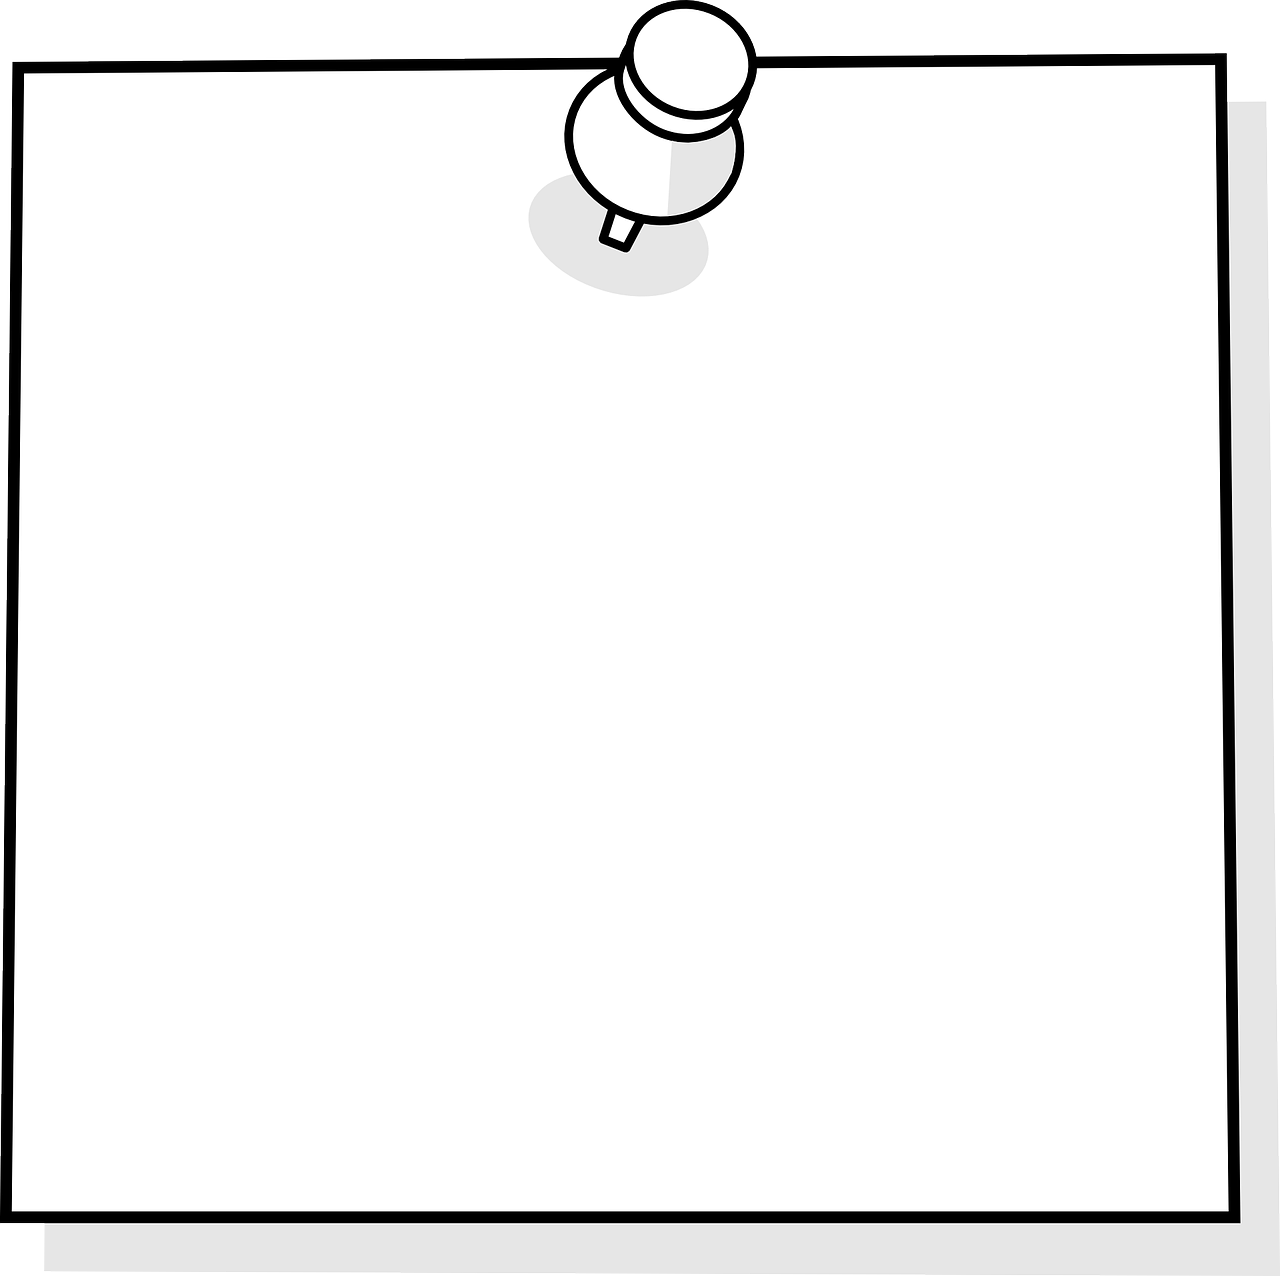
\includegraphics[width=0.7\columnwidth]{figs/example.png}
    \caption{MVSIM Simulation Interface}
    \label{fig:MVSIM}
\end{figure}
\section{Experiment}

\section{Results}




\subsection{Equations}
Punctuate equations with commas or periods when they are part of a sentence, as in

$$
\alpha + \beta = \chi \eqno{(1)}
$$

Note that the equation is centered using a center tab stop. Be sure that the symbols in your equation have been defined before or immediately following the equation. Use (1), not Eq. (1) or equation (1), except at the beginning of a sentence: Equation (1) is . . .


\begin{table}[h]
\caption{An Example of a Table}
\label{tab:example}
\begin{center}
\begin{tabular}{|c||c|c|c|c|c|}
\hline
Tool & \% CPU & RAM & Languages & ROS 2 & Multi-Robot\\ \hline
MVSIM & $-$ & $-$ & C++/Python & \checkmark & \checkmark\\ \hline
Gazebo & $-$ & $-$ & C++ & \checkmark & \checkmark\\ \hline
Webots & $-$ & $-$ & C++/Python & ext. lib. & \checkmark\\ \hline
\end{tabular}
\end{center}
\end{table}


\section{CONCLUSIONS}
Summary, discussion and future work


\addtolength{\textheight}{-12cm}   % This command serves to balance the column lengths
                                  % on the last page of the document manually. It shortens
                                  % the textheight of the last page by a suitable amount.
                                  % This command does not take effect until the next page
                                  % so it should come on the page before the last. Make
                                  % sure that you do not shorten the textheight too much.



%%%%%%%%%%%%%%%%%%%%%%%%%%%%%%%%%%%%%%%%%%%%%%%%%%%%%%%%%%%%%%%%%%%%%%%%%%%%%%%%
% \section*{APPENDIX}

% Appendixes should appear before the acknowledgment.

\section*{ACKNOWLEDGMENT}

The preferred spelling of the word acknowledgment in America is without an e after the g. Avoid the stilted expression, One of us (R. B. G.) thanks . . .  Instead, try R. B. G. thanks. Put sponsor acknowledgments in the unnumbered footnote on the first page.


%%%%%%%%%%%%%%%%%%%%%%%%%%%%%%%%%%%%%%%%%%%%%%%%%%%%%%%%%%%%%%%%%%%%%%%%%%%%%%%%

\bibliographystyle{IEEEtran}
\bibliography{references.bib}

\end{document}
